% arara: pdflatex
\documentclass[tikz,border=0pt]{standalone}
\usepackage{pgfplots}
\usepackage{xcolor}

\begin{document}

\begin{tikzpicture}
  [
    rec0/.style={shade,
                rectangle,
                minimum width=1.5mm,
                minimum height=0.50mm,
                inner sep=0pt,
                outer sep=0pt,
                top color=gray!60!white,
                bottom color=gray!30!white,
                draw=black, 
                very thin},
    rec16/.style={shade,
                rectangle,
                rotate=16,
                minimum width=1.5mm,
                minimum height=0.5mm,
                inner sep=0pt,
                outer sep=0pt,
                top color=gray!60!white,
                bottom color=gray!30!white,
                draw=black, 
                very thin},
    rec16r/.style={shade,
                rectangle,
                rotate=-16,
                minimum width=1.5mm,
                minimum height=0.5mm,
                inner sep=0pt,
                outer sep=0pt,
                top color=gray!60!white,
                bottom color=gray!30!white,
                draw=black, 
                very thin},
    rec45/.style={shade,
                rectangle,
                rotate=45,
                minimum width=14mm,
                minimum height=4.50mm,
                inner sep=0pt,
                outer sep=0pt,
                top color=gray!60!white,
                bottom color=gray!30!white,
                draw=black, 
                very thin}
  ]
% width is 8.64cm
%\newcommand{\figwidth}{8.64cm}
\newcommand{\figwidth}{12.65cm}
\newcommand{\figheight}{8.50cm}

\draw[use as bounding box, white] (0,0) rectangle (\figwidth,\figheight);

% Setup
\begin{scope}[
    xshift=1.75cm,
    yshift=6.00cm,
    ]
    \node[inner sep=0pt]  at (0,0)
        {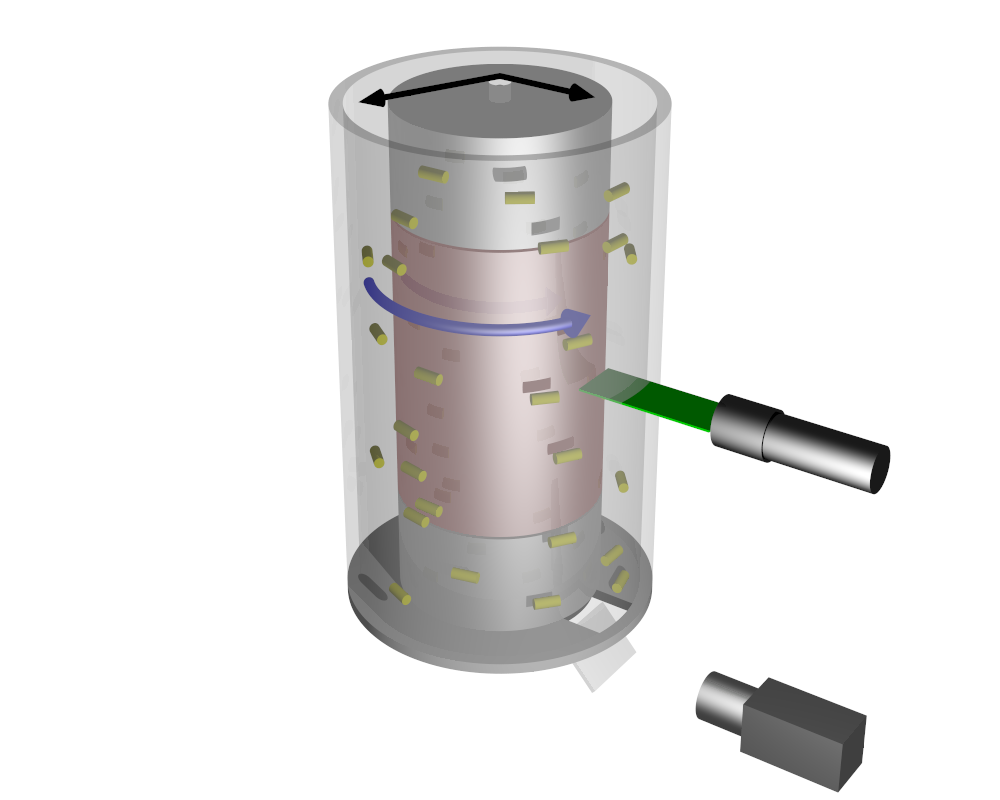
\includegraphics[
            height=5.60cm,
            trim={5cm, 0.25cm, 3.8cm, 0}, 
            clip
        ]{t3csetup.png}};

    \node at (-0.20, 0.70) {\large$\omega_i$};
    \node at (0.20, 2.37) {\large$r_i$};
    \node at (-0.70, 2.35) {\large$r_o$};
\end{scope}

% Still image
\begin{scope}[
    xshift=8.7cm,
    yshift=6.00cm
    ]
    \node[inner sep=0pt] (image) at (0,0)
    {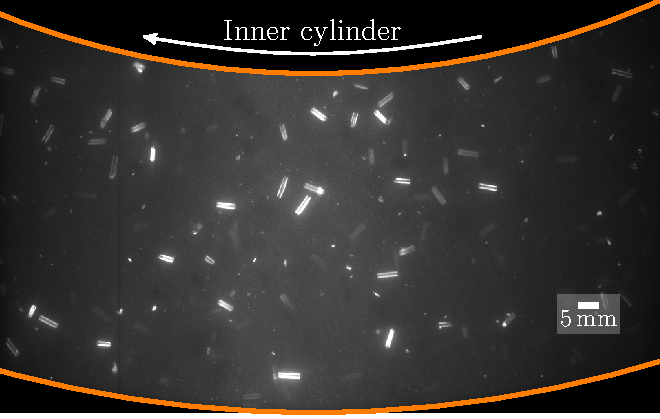
\includegraphics[height=5cm]{figure2image.pdf}};

\end{scope}

% Cylinder
\begin{scope}[
     xshift=3.42cm,
     yshift=8.35cm,
     scale=4.50,
     every node/.append style={transform shape},
    ]
    \clip (-0.487, -1.220) rectangle (0.502, -1.86);

    % Outer cylinder and water inside
    \draw[color=black, fill=white, thin] (0, 0) circle (1.851);

    % inner cylinder
    \draw[color=black, fill=gray!10, thin] (0, 0) circle (1.325);

    \draw[color=black, dashed, thick] (-0.487, -1.25) -- (-0.487, -1.79);
    \draw[color=black, dashed, thick] (0.502, -1.243) -- (0.502, -1.79);
    \draw[color=black, dashed, thick] (-0.487, -1.220) -- (0.502, -1.220);
    \node at (0.025, -1.275) {\scalebox{0.20}{IC}};

    % dashed center line
    \draw[color=red, thick, densely dotted] (0, 0) circle (1.588);

    % filled polygon
    \coordinate (L1) at (-0.487, -1.79);
    \coordinate (L2) at (-0.487, -1.233);
    \coordinate (L3) at (-0.360, -1.275);
    \fill[color=red, opacity=0.2] (L1) -- (L2) -- (L3) -- cycle;
    \coordinate (R1) at (0.502, -1.79);
    \coordinate (R2) at (0.502, -1.228);
    \coordinate (R3) at (0.375, -1.272);
    \fill[color=red, opacity=0.2] (R1) -- (R2) -- (R3) -- cycle;

    \path (0, -1.588) coordinate[rec0];  
    \path (0.4, -1.534) coordinate[rec16];  
    \path (-0.4, -1.534) coordinate[rec16r];  
 \end{scope}

\begin{scope}[
     xshift=9.52cm,
     yshift=8.595cm,
     scale=4.50,
     every node/.append style={transform shape},
    ]
    \clip (-0.487, -1.220) rectangle (0.502, -1.86);
    \draw[color=red, thick, densely dotted] (0, 0) circle (1.588);
 \end{scope}

% big fiber representation
\newcommand{\opas}{0.7}
\begin{scope}[
     xshift=9.70cm,
     yshift=4.6cm,
     scale=0.9,
    ]
    \path[opacity=\opas] (0, -3.50) coordinate[rec45];  
    \draw[color=black, densely dashed, thick, opacity=\opas] (-1.5, -5) -- (1.10, -2.4);
    \draw[->, color=blue,  very thick, >=stealth] (0, -3.5) -- (-0.85, -4.35);
    \draw[color=black, thick, opacity=\opas] (-2, -3.5) -- (2.00, -3.5);
    \draw[color=blue] (-1.5, -3.5) arc (180:225:15mm);
    \node at (-1.70, -4.25) {\scalebox{1.1}{$\theta_p$}};
    \node at (-0.60, -4.5) {\scalebox{1.1}{$p_i$}};
\end{scope}
    
    % labels
\node at (0.20cm, 8.25cm) {\textbf{A}};
\node at (4.45cm, 8.25cm) {\textbf{B}};
\node at (0.90cm, 2.80cm) {\textbf{C}};
\node at (7.20cm, 2.80cm) {\textbf{D}};


\end{tikzpicture}
\end{document}
